\section{{\IterComp}} % and its Space Exploration}

In this section, we present the basic concepts of {\itercomp} and discuss some of the early work on this research topic.
We also consider some of the challenges on reducing its compilation time.
% and present recent work that addresses these challenges.

{\Itercomp} is a well-known compilation technique that searches the optimisation space in order to find the best optimisation for a particular program.
{\Itercomp} is capable of automatically adapting to new platforms, programs, and workloads, in a systematic way.
% while still having a systematic and simple optimisation process.
It works by repeatedly evaluating a large number of compiler optimisations, by means of an execution-driven search, until the best optimisation is found for a particular program~\citep{kisuki99,fursin07,chen10}.
%The main challenge concerning {\itercomp} is the need for efficiently exploring such a large optimisation space~\citep{fursin07,cavazos07,zhou12}.

Figure~\ref{fig:itercomp-diagram} shows an overview of the architecture necessary for performing {\itercomp}.
Given an optimisation setting, a new version of the program is generated.
After profiling the execution of the optimised program, the profiling data is used to produce another optimisation setting for the iterative search.
This profiling data can be as simple as the program's execution time, or more complex, including hardware performance counters for cache behaviour, measurements of energy consumption, etc.
The evaluator can use the feed-back to rank the optimisations and select the best one.
The optimisation generator can be a fixed sequence of optimisations with different tuning parameters or a dynamic mechanism for suggesting a new sequence of optimisation passes.

\begin{figure}[htb]
    \centering
    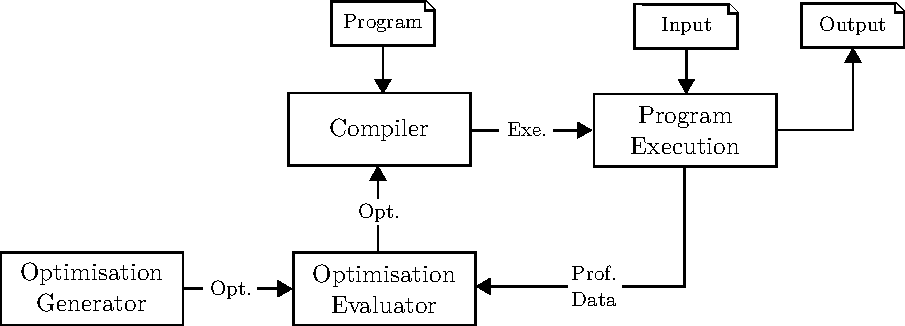
\includegraphics[width=0.8\linewidth]{src/background/figs/itercomp-diagram}
    \caption{A simplified overview of the architecture of an iterative compiler.}
    \label{fig:itercomp-diagram}
\end{figure}

Early work on {\itercomp} has demonstrated its use for determining simultaneously optimal tile sizes and unroll factors for any given loop nest~\cite{kisuki00,knijnenburg04}.
These two transformations are highly interdependent with a very irregular optimisation space, as both of them affect, in different ways, cache behaviour and instruction-level parallelism.
Because of their close interaction, with non-trivial trade-offs, designing a static cost model, that enables the compiler to automatically select the best configuration, is a very laborious and impractical task.
\cite{kisuki00} propose the use of {\itercomp} to address this problem, where it is able to outperform several static techniques.
However, its success comes at the cost of a significant increase in compilation time, which involves several runs of the program for the execution-driven search.

Despite the high cost of compilation time, there are scenarios where this approach is highly attractive due to high-performance requirements, such as embedded systems and library codes.
Moreover, {\itercomp} was originally intended to be applied in an \textit{offline} scenario, where the software vendor optimises the program before shipping, the compilation time can be amortised across the number of products shipped, the lifetime of the product, or a much larger number of executions in production~\cite{kisuki99,kisuki00,chen10}.
It is also useful in contexts where the underlying architecture changes frequently, as the iterative search dismisses the arduous task of manually optimising the program for the new platform.

Numerous researchers have addressed the problem of reducing the optimisation space.
For the same problem of selecting optimal tile sizes and unroll factors, \cite{knijnenburg04} suggest the use of a cache model to avoid executing candidates during the execution-driven search of {\itercomp}.
By querying the cache model, the compiler is able to rank the optimisation candidates, filtering out candidates below a given threshold.
Their results show that it is possible to reduce the number of executions by up to about 70\%, without a significant degradation of the resulting optimisation.

\cite{agakov06} suggest using machine learning techniques to speed up {\itercomp}.
They propose a mechanism that learns a predictive model from a training set of benchmarks.
This predictive model will later be used for predicting regions of the optimisation space that are more likely to contain promising results.
Their approach is able to significantly reduce the number of executions necessary for achieving good performance improvements with the iterative search.

More recently, \cite{ogilvie17} have proposed a strategy based on active learning techniques to focus the search on promising optimisation candidates.
It avoids redundant candidates 
by using high-quality models which based on a combination of optimisation settings to predict the runtime of the training benchmarks.

The problem of reducing the optimisation space is out of the scope of this thesis.
Having a better search strategy would only improve our mechanism for online {\itercomp}.

